\documentclass[1p]{elsarticle_modified}
%\bibliographystyle{elsarticle-num}

%\usepackage[colorlinks]{hyperref}
%\usepackage{abbrmath_seonhwa} %\Abb, \Ascr, \Acal ,\Abf, \Afrak
\usepackage{amsfonts}
\usepackage{amssymb}
\usepackage{amsmath}
\usepackage{amsthm}
\usepackage{scalefnt}
\usepackage{amsbsy}
\usepackage{kotex}
\usepackage{caption}
\usepackage{subfig}
\usepackage{color}
\usepackage{graphicx}
\usepackage{xcolor} %% white, black, red, green, blue, cyan, magenta, yellow
\usepackage{float}
\usepackage{setspace}
\usepackage{hyperref}

\usepackage{tikz}
\usetikzlibrary{arrows}

\usepackage{multirow}
\usepackage{array} % fixed length table
\usepackage{hhline}

%%%%%%%%%%%%%%%%%%%%%
\makeatletter
\renewcommand*\env@matrix[1][\arraystretch]{%
	\edef\arraystretch{#1}%
	\hskip -\arraycolsep
	\let\@ifnextchar\new@ifnextchar
	\array{*\c@MaxMatrixCols c}}
\makeatother %https://tex.stackexchange.com/questions/14071/how-can-i-increase-the-line-spacing-in-a-matrix
%%%%%%%%%%%%%%%

\usepackage[normalem]{ulem}

\newcommand{\msout}[1]{\ifmmode\text{\sout{\ensuremath{#1}}}\else\sout{#1}\fi}
%SOURCE: \msout is \stkout macro in https://tex.stackexchange.com/questions/20609/strikeout-in-math-mode

\newcommand{\cancel}[1]{
	\ifmmode
	{\color{red}\msout{#1}}
	\else
	{\color{red}\sout{#1}}
	\fi
}

\newcommand{\add}[1]{
	{\color{blue}\uwave{#1}}
}

\newcommand{\replace}[2]{
	\ifmmode
	{\color{red}\msout{#1}}{\color{blue}\uwave{#2}}
	\else
	{\color{red}\sout{#1}}{\color{blue}\uwave{#2}}
	\fi
}

\newcommand{\Sol}{\mathcal{S}} %segment
\newcommand{\D}{D} %diagram
\newcommand{\A}{\mathcal{A}} %arc


%%%%%%%%%%%%%%%%%%%%%%%%%%%%%5 test

\def\sl{\operatorname{\textup{SL}}(2,\Cbb)}
\def\psl{\operatorname{\textup{PSL}}(2,\Cbb)}
\def\quan{\mkern 1mu \triangleright \mkern 1mu}

\theoremstyle{definition}
\newtheorem{thm}{Theorem}[section]
\newtheorem{prop}[thm]{Proposition}
\newtheorem{lem}[thm]{Lemma}
\newtheorem{ques}[thm]{Question}
\newtheorem{cor}[thm]{Corollary}
\newtheorem{defn}[thm]{Definition}
\newtheorem{exam}[thm]{Example}
\newtheorem{rmk}[thm]{Remark}
\newtheorem{alg}[thm]{Algorithm}

\newcommand{\I}{\sqrt{-1}}
\begin{document}

%\begin{frontmatter}
%
%\title{Boundary parabolic representations of knots up to 8 crossings}
%
%%% Group authors per affiliation:
%\author{Yunhi Cho} 
%\address{Department of Mathematics, University of Seoul, Seoul, Korea}
%\ead{yhcho@uos.ac.kr}
%
%
%\author{Seonhwa Kim} %\fnref{s_kim}}
%\address{Center for Geometry and Physics, Institute for Basic Science, Pohang, 37673, Korea}
%\ead{ryeona17@ibs.re.kr}
%
%\author{Hyuk Kim}
%\address{Department of Mathematical Sciences, Seoul National University, Seoul 08826, Korea}
%\ead{hyukkim@snu.ac.kr}
%
%\author{Seokbeom Yoon}
%\address{Department of Mathematical Sciences, Seoul National University, Seoul, 08826,  Korea}
%\ead{sbyoon15@snu.ac.kr}
%
%\begin{abstract}
%We find all boundary parabolic representation of knots up to 8 crossings.
%
%\end{abstract}
%\begin{keyword}
%    \MSC[2010] 57M25 
%\end{keyword}
%
%\end{frontmatter}

%\linenumbers
%\tableofcontents
%
\newcommand\colored[1]{\textcolor{white}{\rule[-0.35ex]{0.8em}{1.4ex}}\kern-0.8em\color{red} #1}%
%\newcommand\colored[1]{\textcolor{white}{ #1}\kern-2.17ex	\textcolor{white}{ #1}\kern-1.81ex	\textcolor{white}{ #1}\kern-2.15ex\color{red}#1	}

{\Large $\underline{12a_{1265}~(K12a_{1265})}$}

\setlength{\tabcolsep}{10pt}
\renewcommand{\arraystretch}{1.6}
\vspace{1cm}\begin{tabular}{m{100pt}>{\centering\arraybackslash}m{274pt}}
\multirow{5}{120pt}{
	\centering
	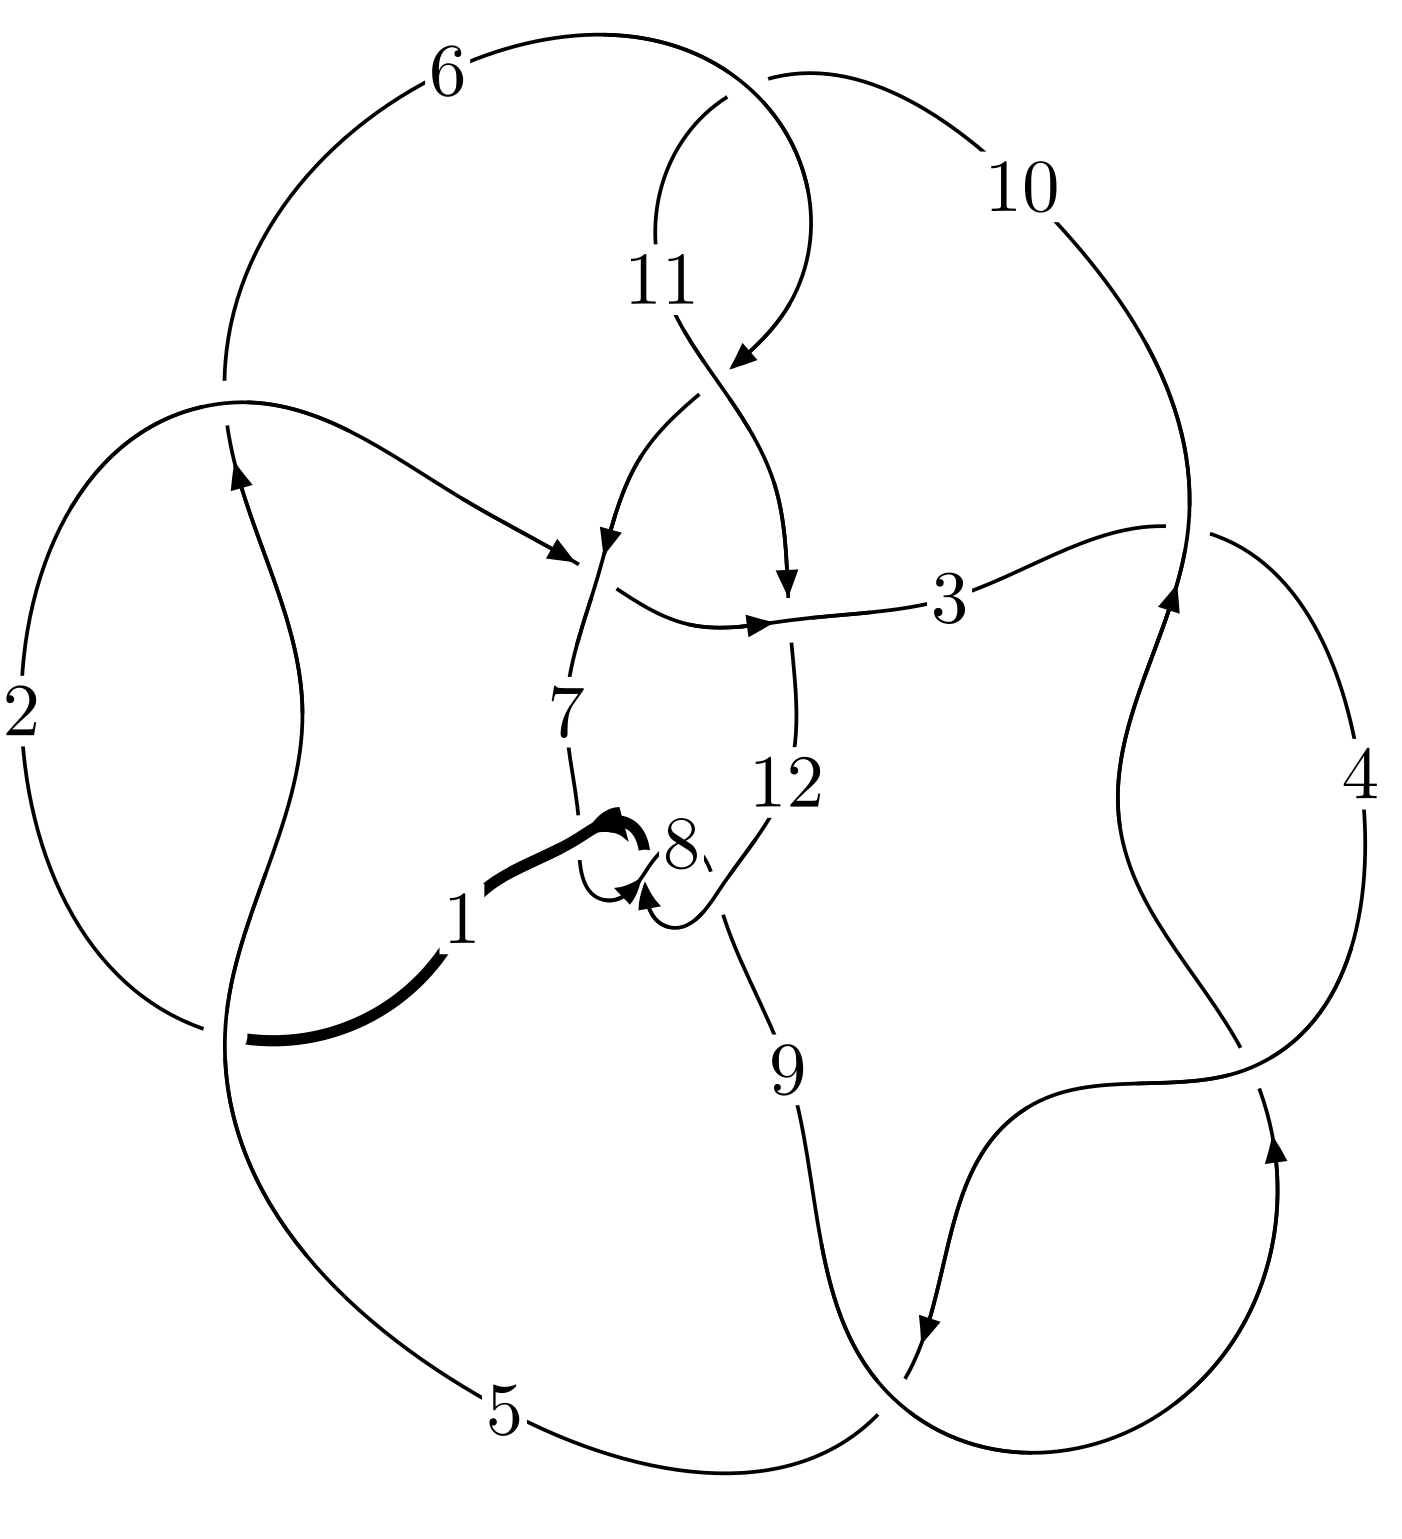
\includegraphics[width=112pt]{../../../GIT/diagram.site/Diagrams/png/2066_12a_1265.png}\\
\ \ \ A knot diagram\footnotemark}&
\allowdisplaybreaks
\textbf{Linearized knot diagam} \\
\cline{2-2}
 &
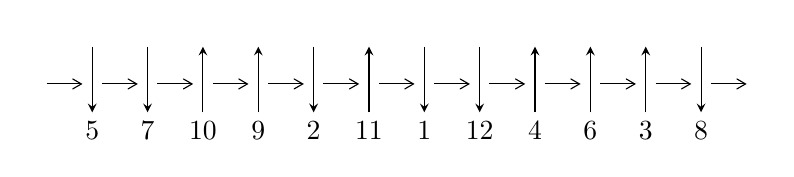
\begin{tikzpicture}[x=20pt, y=17pt]
	% nodes
	\node (C0) at (0, 0) {};
	\node (C1) at (1, 0) {};
	\node (C1U) at (1, +1) {};
	\node (C1D) at (1, -1) {5};

	\node (C2) at (2, 0) {};
	\node (C2U) at (2, +1) {};
	\node (C2D) at (2, -1) {7};

	\node (C3) at (3, 0) {};
	\node (C3U) at (3, +1) {};
	\node (C3D) at (3, -1) {10};

	\node (C4) at (4, 0) {};
	\node (C4U) at (4, +1) {};
	\node (C4D) at (4, -1) {9};

	\node (C5) at (5, 0) {};
	\node (C5U) at (5, +1) {};
	\node (C5D) at (5, -1) {2};

	\node (C6) at (6, 0) {};
	\node (C6U) at (6, +1) {};
	\node (C6D) at (6, -1) {11};

	\node (C7) at (7, 0) {};
	\node (C7U) at (7, +1) {};
	\node (C7D) at (7, -1) {1};

	\node (C8) at (8, 0) {};
	\node (C8U) at (8, +1) {};
	\node (C8D) at (8, -1) {12};

	\node (C9) at (9, 0) {};
	\node (C9U) at (9, +1) {};
	\node (C9D) at (9, -1) {4};

	\node (C10) at (10, 0) {};
	\node (C10U) at (10, +1) {};
	\node (C10D) at (10, -1) {6};

	\node (C11) at (11, 0) {};
	\node (C11U) at (11, +1) {};
	\node (C11D) at (11, -1) {3};

	\node (C12) at (12, 0) {};
	\node (C12U) at (12, +1) {};
	\node (C12D) at (12, -1) {8};
	\node (C13) at (13, 0) {};

	% arrows
	\draw[->,>={angle 60}]
	(C0) edge (C1) (C1) edge (C2) (C2) edge (C3) (C3) edge (C4) (C4) edge (C5) (C5) edge (C6) (C6) edge (C7) (C7) edge (C8) (C8) edge (C9) (C9) edge (C10) (C10) edge (C11) (C11) edge (C12) (C12) edge (C13) ;	\draw[->,>=stealth]
	(C1U) edge (C1D) (C2U) edge (C2D) (C3D) edge (C3U) (C4D) edge (C4U) (C5U) edge (C5D) (C6D) edge (C6U) (C7U) edge (C7D) (C8U) edge (C8D) (C9D) edge (C9U) (C10D) edge (C10U) (C11D) edge (C11U) (C12U) edge (C12D) ;
	\end{tikzpicture} \\
\hhline{~~} \\& 
\textbf{Solving Sequence} \\ \cline{2-2} 
 &
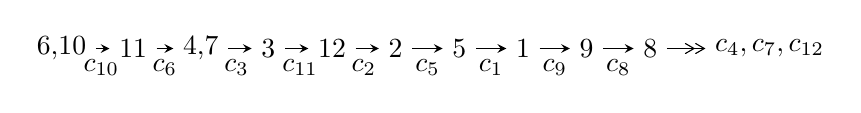
\begin{tikzpicture}[x=23pt, y=7pt]
	% node
	\node (A0) at (-1/8, 0) {6,10};
	\node (A1) at (1, 0) {11};
	\node (A2) at (33/16, 0) {4,7};
	\node (A3) at (25/8, 0) {3};
	\node (A4) at (33/8, 0) {12};
	\node (A5) at (41/8, 0) {2};
	\node (A6) at (49/8, 0) {5};
	\node (A7) at (57/8, 0) {1};
	\node (A8) at (65/8, 0) {9};
	\node (A9) at (73/8, 0) {8};
	\node (C1) at (1/2, -1) {$c_{10}$};
	\node (C2) at (3/2, -1) {$c_{6}$};
	\node (C3) at (21/8, -1) {$c_{3}$};
	\node (C4) at (29/8, -1) {$c_{11}$};
	\node (C5) at (37/8, -1) {$c_{2}$};
	\node (C6) at (45/8, -1) {$c_{5}$};
	\node (C7) at (53/8, -1) {$c_{1}$};
	\node (C8) at (61/8, -1) {$c_{9}$};
	\node (C9) at (69/8, -1) {$c_{8}$};
	\node (A10) at (11, 0) {$c_{4},c_{7},c_{12}$};

	% edge
	\draw[->,>=stealth]	
	(A0) edge (A1) (A1) edge (A2) (A2) edge (A3) (A3) edge (A4) (A4) edge (A5) (A5) edge (A6) (A6) edge (A7) (A7) edge (A8) (A8) edge (A9) ;
	\draw[->>,>={angle 60}]	
	(A9) edge (A10);
\end{tikzpicture} \\ 

\end{tabular} \\

\footnotetext{
The image of knot diagram is generated by the software ``\textbf{Draw programme}" developed by Andrew Bartholomew(\url{http://www.layer8.co.uk/maths/draw/index.htm\#Running-draw}), where we modified some parts for our purpose(\url{https://github.com/CATsTAILs/LinksPainter}).
}\phantom \\ \newline 
\centering \textbf{Ideals for irreducible components\footnotemark of $X_{\text{par}}$} 
 
\begin{align*}
I^u_{1}&=\langle 
2.07379\times10^{255} u^{108}-2.75072\times10^{255} u^{107}+\cdots+1.59536\times10^{256} b-5.93025\times10^{255},\\
\phantom{I^u_{1}}&\phantom{= \langle  }-2.85670\times10^{255} u^{108}-2.09806\times10^{255} u^{107}+\cdots+1.59536\times10^{256} a+1.89502\times10^{257},\\
\phantom{I^u_{1}}&\phantom{= \langle  }u^{109}- u^{108}+\cdots-11 u-1\rangle \\
I^u_{2}&=\langle 
-61909880 u^{26}-37523313 u^{25}+\cdots+242539 b-102346633,\\
\phantom{I^u_{2}}&\phantom{= \langle  }-121965917 u^{26}-75233918 u^{25}+\cdots+242539 a-193272722,\;u^{27}-6 u^{25}+\cdots+9 u^2-1\rangle \\
\\
\end{align*}
\raggedright * 2 irreducible components of $\dim_{\mathbb{C}}=0$, with total 136 representations.\\
\footnotetext{All coefficients of polynomials are rational numbers. But the coefficients are sometimes approximated in decimal forms when there is not enough margin.}
\newpage
\renewcommand{\arraystretch}{1}
\centering \section*{I. $I^u_{1}= \langle 2.07\times10^{255} u^{108}-2.75\times10^{255} u^{107}+\cdots+1.60\times10^{256} b-5.93\times10^{255},\;-2.86\times10^{255} u^{108}-2.10\times10^{255} u^{107}+\cdots+1.60\times10^{256} a+1.90\times10^{257},\;u^{109}- u^{108}+\cdots-11 u-1 \rangle$}
\flushleft \textbf{(i) Arc colorings}\\
\begin{tabular}{m{7pt} m{180pt} m{7pt} m{180pt} }
\flushright $a_{6}=$&$\begin{pmatrix}0\\u\end{pmatrix}$ \\
\flushright $a_{10}=$&$\begin{pmatrix}1\\0\end{pmatrix}$ \\
\flushright $a_{11}=$&$\begin{pmatrix}1\\- u^2\end{pmatrix}$ \\
\flushright $a_{4}=$&$\begin{pmatrix}0.179063 u^{108}+0.131510 u^{107}+\cdots-1.04736 u-11.8784\\-0.129989 u^{108}+0.172420 u^{107}+\cdots-0.912281 u+0.371719\end{pmatrix}$ \\
\flushright $a_{7}=$&$\begin{pmatrix}u\\- u^3+u\end{pmatrix}$ \\
\flushright $a_{3}=$&$\begin{pmatrix}0.309052 u^{108}-0.0409100 u^{107}+\cdots-0.135083 u-12.2501\\-0.129989 u^{108}+0.172420 u^{107}+\cdots-0.912281 u+0.371719\end{pmatrix}$ \\
\flushright $a_{12}=$&$\begin{pmatrix}-3.71909 u^{108}+4.03133 u^{107}+\cdots-6.89095 u+6.17203\\-1.53240 u^{108}+0.953587 u^{107}+\cdots-4.61684 u-0.402304\end{pmatrix}$ \\
\flushright $a_{2}=$&$\begin{pmatrix}0.631835 u^{108}-0.198694 u^{107}+\cdots-0.0460130 u-12.1832\\-0.0170239 u^{108}+0.114081 u^{107}+\cdots-2.96097 u+0.273605\end{pmatrix}$ \\
\flushright $a_{5}=$&$\begin{pmatrix}0.688228 u^{108}+0.412394 u^{107}+\cdots+34.8906 u-11.0803\\0.406094 u^{108}+0.104249 u^{107}+\cdots+5.65327 u+1.03987\end{pmatrix}$ \\
\flushright $a_{1}=$&$\begin{pmatrix}3.60935 u^{108}-4.32794 u^{107}+\cdots-4.82469 u+3.17695\\1.46357 u^{108}-0.289308 u^{107}+\cdots+18.8077 u+1.37757\end{pmatrix}$ \\
\flushright $a_{9}=$&$\begin{pmatrix}2.37268 u^{108}-1.78944 u^{107}+\cdots+4.90531 u-4.99223\\0.330824 u^{108}-0.403588 u^{107}+\cdots-4.64106 u-0.253700\end{pmatrix}$ \\
\flushright $a_{8}=$&$\begin{pmatrix}-0.0243952 u^{108}+2.39013 u^{107}+\cdots+51.8115 u+3.31575\\-0.617749 u^{108}+1.05009 u^{107}+\cdots-10.7866 u-0.532978\end{pmatrix}$\\&\end{tabular}
\flushleft \textbf{(ii) Obstruction class $= -1$}\\~\\
\flushleft \textbf{(iii) Cusp Shapes $= 0.197018 u^{108}-0.211745 u^{107}+\cdots-32.0632 u-8.93887$}\\~\\
\newpage\renewcommand{\arraystretch}{1}
\flushleft \textbf{(iv) u-Polynomials at the component}\newline \\
\begin{tabular}{m{50pt}|m{274pt}}
Crossings & \hspace{64pt}u-Polynomials at each crossing \\
\hline $$\begin{aligned}c_{1},c_{5}\end{aligned}$$&$\begin{aligned}
&u^{109}-37 u^{107}+\cdots+59522 u+7979
\end{aligned}$\\
\hline $$\begin{aligned}c_{2}\end{aligned}$$&$\begin{aligned}
&u^{109}- u^{108}+\cdots+8276 u+1297
\end{aligned}$\\
\hline $$\begin{aligned}c_{3},c_{4},c_{9}\end{aligned}$$&$\begin{aligned}
&u^{109}+u^{108}+\cdots+256 u+32
\end{aligned}$\\
\hline $$\begin{aligned}c_{6},c_{10}\end{aligned}$$&$\begin{aligned}
&u^{109}+u^{108}+\cdots-11 u+1
\end{aligned}$\\
\hline $$\begin{aligned}c_{7},c_{8},c_{12}\end{aligned}$$&$\begin{aligned}
&u^{109}+2 u^{108}+\cdots-1969 u-419
\end{aligned}$\\
\hline $$\begin{aligned}c_{11}\end{aligned}$$&$\begin{aligned}
&u^{109}-7 u^{108}+\cdots+35263 u+3563
\end{aligned}$\\
\hline
\end{tabular}\\~\\
\newpage\renewcommand{\arraystretch}{1}
\flushleft \textbf{(v) Riley Polynomials at the component}\newline \\
\begin{tabular}{m{50pt}|m{274pt}}
Crossings & \hspace{64pt}Riley Polynomials at each crossing \\
\hline $$\begin{aligned}c_{1},c_{5}\end{aligned}$$&$\begin{aligned}
&y^{109}-74 y^{108}+\cdots+1156541080 y-63664441
\end{aligned}$\\
\hline $$\begin{aligned}c_{2}\end{aligned}$$&$\begin{aligned}
&y^{109}+13 y^{108}+\cdots-254211800 y-1682209
\end{aligned}$\\
\hline $$\begin{aligned}c_{3},c_{4},c_{9}\end{aligned}$$&$\begin{aligned}
&y^{109}+109 y^{108}+\cdots+137216 y-1024
\end{aligned}$\\
\hline $$\begin{aligned}c_{6},c_{10}\end{aligned}$$&$\begin{aligned}
&y^{109}-55 y^{108}+\cdots+109 y-1
\end{aligned}$\\
\hline $$\begin{aligned}c_{7},c_{8},c_{12}\end{aligned}$$&$\begin{aligned}
&y^{109}+104 y^{108}+\cdots+3301255 y-175561
\end{aligned}$\\
\hline $$\begin{aligned}c_{11}\end{aligned}$$&$\begin{aligned}
&y^{109}-7 y^{108}+\cdots+969448839 y-12694969
\end{aligned}$\\
\hline
\end{tabular}\\~\\
\newpage\flushleft \textbf{(vi) Complex Volumes and Cusp Shapes}
$$\begin{array}{c|c|c}  
\text{Solutions to }I^u_{1}& \I (\text{vol} + \sqrt{-1}CS) & \text{Cusp shape}\\
 \hline 
\begin{aligned}
u &= \phantom{-}0.917295 + 0.388841 I \\
a &= -2.97771 + 0.64132 I \\
b &= -0.062160 + 1.316590 I\end{aligned}
 & -1.67290 - 3.11299 I & \phantom{-0.000000 } 0 \\ \hline\begin{aligned}
u &= \phantom{-}0.917295 - 0.388841 I \\
a &= -2.97771 - 0.64132 I \\
b &= -0.062160 - 1.316590 I\end{aligned}
 & -1.67290 + 3.11299 I & \phantom{-0.000000 } 0 \\ \hline\begin{aligned}
u &= \phantom{-}0.228541 + 0.969277 I \\
a &= \phantom{-}0.403082 - 0.308766 I \\
b &= \phantom{-}0.541312 - 0.401025 I\end{aligned}
 & -2.94127 - 3.17384 I & \phantom{-0.000000 } 0 \\ \hline\begin{aligned}
u &= \phantom{-}0.228541 - 0.969277 I \\
a &= \phantom{-}0.403082 + 0.308766 I \\
b &= \phantom{-}0.541312 + 0.401025 I\end{aligned}
 & -2.94127 + 3.17384 I & \phantom{-0.000000 } 0 \\ \hline\begin{aligned}
u &= -0.888968 + 0.445422 I \\
a &= \phantom{-}1.71464 + 0.48468 I \\
b &= -0.45791 + 1.36846 I\end{aligned}
 & -2.11543 - 7.53198 I & \phantom{-0.000000 } 0 \\ \hline\begin{aligned}
u &= -0.888968 - 0.445422 I \\
a &= \phantom{-}1.71464 - 0.48468 I \\
b &= -0.45791 - 1.36846 I\end{aligned}
 & -2.11543 + 7.53198 I & \phantom{-0.000000 } 0 \\ \hline\begin{aligned}
u &= \phantom{-}0.877149 + 0.430029 I \\
a &= -1.90212 + 0.77696 I \\
b &= \phantom{-}0.28424 + 1.48490 I\end{aligned}
 & -7.93888 + 4.00907 I & \phantom{-0.000000 } 0 \\ \hline\begin{aligned}
u &= \phantom{-}0.877149 - 0.430029 I \\
a &= -1.90212 - 0.77696 I \\
b &= \phantom{-}0.28424 - 1.48490 I\end{aligned}
 & -7.93888 - 4.00907 I & \phantom{-0.000000 } 0 \\ \hline\begin{aligned}
u &= -0.888800 + 0.394316 I \\
a &= \phantom{-}2.55286 + 1.03132 I \\
b &= -0.04364 + 1.44473 I\end{aligned}
 & -7.67955 - 0.12193 I & \phantom{-0.000000 } 0 \\ \hline\begin{aligned}
u &= -0.888800 - 0.394316 I \\
a &= \phantom{-}2.55286 - 1.03132 I \\
b &= -0.04364 - 1.44473 I\end{aligned}
 & -7.67955 + 0.12193 I & \phantom{-0.000000 } 0\\
 \hline 
 \end{array}$$\newpage$$\begin{array}{c|c|c}  
\text{Solutions to }I^u_{1}& \I (\text{vol} + \sqrt{-1}CS) & \text{Cusp shape}\\
 \hline 
\begin{aligned}
u &= \phantom{-}0.995644 + 0.311398 I \\
a &= \phantom{-}0.706710 - 0.278460 I \\
b &= -0.409925 + 0.785108 I\end{aligned}
 & \phantom{-}8.58686 + 1.56893 I & \phantom{-0.000000 } 0 \\ \hline\begin{aligned}
u &= \phantom{-}0.995644 - 0.311398 I \\
a &= \phantom{-}0.706710 + 0.278460 I \\
b &= -0.409925 - 0.785108 I\end{aligned}
 & \phantom{-}8.58686 - 1.56893 I & \phantom{-0.000000 } 0 \\ \hline\begin{aligned}
u &= -0.951558 + 0.088021 I \\
a &= -0.804740 + 0.333709 I \\
b &= \phantom{-}0.351609 + 0.845050 I\end{aligned}
 & \phantom{-}1.361510 - 0.218866 I & \phantom{-0.000000 } 0 \\ \hline\begin{aligned}
u &= -0.951558 - 0.088021 I \\
a &= -0.804740 - 0.333709 I \\
b &= \phantom{-}0.351609 - 0.845050 I\end{aligned}
 & \phantom{-}1.361510 + 0.218866 I & \phantom{-0.000000 } 0 \\ \hline\begin{aligned}
u &= -0.030115 + 0.932446 I \\
a &= -0.41453 - 1.41539 I \\
b &= -0.190470 - 1.327410 I\end{aligned}
 & -3.24398 + 0.72576 I & \phantom{-0.000000 } 0 \\ \hline\begin{aligned}
u &= -0.030115 - 0.932446 I \\
a &= -0.41453 + 1.41539 I \\
b &= -0.190470 + 1.327410 I\end{aligned}
 & -3.24398 - 0.72576 I & \phantom{-0.000000 } 0 \\ \hline\begin{aligned}
u &= -0.177661 + 0.911697 I \\
a &= -0.616810 - 0.190827 I \\
b &= -0.809475 - 0.389422 I\end{aligned}
 & \phantom{-}2.65935 + 7.11690 I & \phantom{-0.000000 } 0 \\ \hline\begin{aligned}
u &= -0.177661 - 0.911697 I \\
a &= -0.616810 + 0.190827 I \\
b &= -0.809475 + 0.389422 I\end{aligned}
 & \phantom{-}2.65935 - 7.11690 I & \phantom{-0.000000 } 0 \\ \hline\begin{aligned}
u &= -0.818616 + 0.425892 I \\
a &= \phantom{-}1.33364 + 1.27306 I \\
b &= -0.07438 + 1.77511 I\end{aligned}
 & -6.74853 - 1.80740 I & \phantom{-0.000000 } 0 \\ \hline\begin{aligned}
u &= -0.818616 - 0.425892 I \\
a &= \phantom{-}1.33364 - 1.27306 I \\
b &= -0.07438 - 1.77511 I\end{aligned}
 & -6.74853 + 1.80740 I & \phantom{-0.000000 } 0\\
 \hline 
 \end{array}$$\newpage$$\begin{array}{c|c|c}  
\text{Solutions to }I^u_{1}& \I (\text{vol} + \sqrt{-1}CS) & \text{Cusp shape}\\
 \hline 
\begin{aligned}
u &= \phantom{-}1.041810 + 0.281133 I \\
a &= \phantom{-}0.195601 - 0.995537 I \\
b &= -0.091742 - 0.730542 I\end{aligned}
 & -0.47156 + 2.62732 I & \phantom{-0.000000 } 0 \\ \hline\begin{aligned}
u &= \phantom{-}1.041810 - 0.281133 I \\
a &= \phantom{-}0.195601 + 0.995537 I \\
b &= -0.091742 + 0.730542 I\end{aligned}
 & -0.47156 - 2.62732 I & \phantom{-0.000000 } 0 \\ \hline\begin{aligned}
u &= \phantom{-}0.841457 + 0.348859 I \\
a &= -2.30224 + 2.55558 I \\
b &= \phantom{-}0.00477 + 1.64810 I\end{aligned}
 & -6.24517 + 1.53642 I & \phantom{-0.000000 } 0 \\ \hline\begin{aligned}
u &= \phantom{-}0.841457 - 0.348859 I \\
a &= -2.30224 - 2.55558 I \\
b &= \phantom{-}0.00477 - 1.64810 I\end{aligned}
 & -6.24517 - 1.53642 I & \phantom{-0.000000 } 0 \\ \hline\begin{aligned}
u &= -1.043380 + 0.349847 I \\
a &= \phantom{-}0.59169 - 1.31110 I \\
b &= \phantom{-}0.213307 - 0.288789 I\end{aligned}
 & \phantom{-}3.76245 - 4.90249 I & \phantom{-0.000000 } 0 \\ \hline\begin{aligned}
u &= -1.043380 - 0.349847 I \\
a &= \phantom{-}0.59169 + 1.31110 I \\
b &= \phantom{-}0.213307 + 0.288789 I\end{aligned}
 & \phantom{-}3.76245 + 4.90249 I & \phantom{-0.000000 } 0 \\ \hline\begin{aligned}
u &= -0.056570 + 0.887294 I \\
a &= \phantom{-}0.23778 - 1.92158 I \\
b &= -0.059940 - 1.405360 I\end{aligned}
 & -5.49952 + 1.73654 I & \phantom{-0.000000 } 0 \\ \hline\begin{aligned}
u &= -0.056570 - 0.887294 I \\
a &= \phantom{-}0.23778 + 1.92158 I \\
b &= -0.059940 + 1.405360 I\end{aligned}
 & -5.49952 - 1.73654 I & \phantom{-0.000000 } 0 \\ \hline\begin{aligned}
u &= \phantom{-}1.035550 + 0.405055 I \\
a &= -0.248386 + 0.014630 I \\
b &= \phantom{-}0.987429 - 0.256543 I\end{aligned}
 & \phantom{-}3.47799 + 0.92445 I & \phantom{-0.000000 } 0 \\ \hline\begin{aligned}
u &= \phantom{-}1.035550 - 0.405055 I \\
a &= -0.248386 - 0.014630 I \\
b &= \phantom{-}0.987429 + 0.256543 I\end{aligned}
 & \phantom{-}3.47799 - 0.92445 I & \phantom{-0.000000 } 0\\
 \hline 
 \end{array}$$\newpage$$\begin{array}{c|c|c}  
\text{Solutions to }I^u_{1}& \I (\text{vol} + \sqrt{-1}CS) & \text{Cusp shape}\\
 \hline 
\begin{aligned}
u &= \phantom{-}0.768950 + 0.400282 I \\
a &= -0.42544 + 1.60470 I \\
b &= -0.15501 + 1.61674 I\end{aligned}
 & -8.31025 - 0.46293 I & \phantom{-0.000000 } 0 \\ \hline\begin{aligned}
u &= \phantom{-}0.768950 - 0.400282 I \\
a &= -0.42544 - 1.60470 I \\
b &= -0.15501 - 1.61674 I\end{aligned}
 & -8.31025 + 0.46293 I & \phantom{-0.000000 } 0 \\ \hline\begin{aligned}
u &= \phantom{-}0.351659 + 1.087250 I \\
a &= -0.14092 + 1.98936 I \\
b &= -0.31351 + 1.47441 I\end{aligned}
 & -3.32481 - 11.20770 I & \phantom{-0.000000 } 0 \\ \hline\begin{aligned}
u &= \phantom{-}0.351659 - 1.087250 I \\
a &= -0.14092 - 1.98936 I \\
b &= -0.31351 - 1.47441 I\end{aligned}
 & -3.32481 + 11.20770 I & \phantom{-0.000000 } 0 \\ \hline\begin{aligned}
u &= -0.779063 + 0.357335 I \\
a &= \phantom{-}0.65483 + 2.72737 I \\
b &= -0.02730 + 1.56178 I\end{aligned}
 & -8.07250 - 3.15214 I & \phantom{-0.000000 -}0. + 9.48648 I \\ \hline\begin{aligned}
u &= -0.779063 - 0.357335 I \\
a &= \phantom{-}0.65483 - 2.72737 I \\
b &= -0.02730 - 1.56178 I\end{aligned}
 & -8.07250 + 3.15214 I & \phantom{-0.000000 } 0. - 9.48648 I \\ \hline\begin{aligned}
u &= -0.748158 + 0.403532 I \\
a &= -0.017264 + 1.191600 I \\
b &= \phantom{-}0.32327 + 1.53971 I\end{aligned}
 & -2.59809 + 3.91150 I & \phantom{-0.000000 } 0 \\ \hline\begin{aligned}
u &= -0.748158 - 0.403532 I \\
a &= -0.017264 - 1.191600 I \\
b &= \phantom{-}0.32327 - 1.53971 I\end{aligned}
 & -2.59809 - 3.91150 I & \phantom{-0.000000 } 0 \\ \hline\begin{aligned}
u &= -1.082180 + 0.405592 I \\
a &= \phantom{-}0.011986 - 0.151685 I \\
b &= -0.846547 - 0.667650 I\end{aligned}
 & -0.19217 - 3.18270 I & \phantom{-0.000000 } 0 \\ \hline\begin{aligned}
u &= -1.082180 - 0.405592 I \\
a &= \phantom{-}0.011986 + 0.151685 I \\
b &= -0.846547 + 0.667650 I\end{aligned}
 & -0.19217 + 3.18270 I & \phantom{-0.000000 } 0\\
 \hline 
 \end{array}$$\newpage$$\begin{array}{c|c|c}  
\text{Solutions to }I^u_{1}& \I (\text{vol} + \sqrt{-1}CS) & \text{Cusp shape}\\
 \hline 
\begin{aligned}
u &= \phantom{-}0.751805 + 0.334380 I \\
a &= -0.00652 + 3.35811 I \\
b &= \phantom{-}0.11632 + 1.47827 I\end{aligned}
 & -2.26710 + 6.30546 I & \phantom{-0.000000 } 0. - 8.32600 I \\ \hline\begin{aligned}
u &= \phantom{-}0.751805 - 0.334380 I \\
a &= -0.00652 - 3.35811 I \\
b &= \phantom{-}0.11632 - 1.47827 I\end{aligned}
 & -2.26710 - 6.30546 I & \phantom{-0.000000 -}0. + 8.32600 I \\ \hline\begin{aligned}
u &= -0.530917 + 1.054470 I \\
a &= -0.160119 - 0.275138 I \\
b &= -0.255742 - 0.184696 I\end{aligned}
 & -1.27003 - 1.78460 I & \phantom{-0.000000 } 0 \\ \hline\begin{aligned}
u &= -0.530917 - 1.054470 I \\
a &= -0.160119 + 0.275138 I \\
b &= -0.255742 + 0.184696 I\end{aligned}
 & -1.27003 + 1.78460 I & \phantom{-0.000000 } 0 \\ \hline\begin{aligned}
u &= \phantom{-}1.132170 + 0.343312 I \\
a &= -0.779850 + 0.293221 I \\
b &= \phantom{-}0.619776 + 0.241214 I\end{aligned}
 & \phantom{-}3.19928 + 3.72682 I & \phantom{-0.000000 } 0 \\ \hline\begin{aligned}
u &= \phantom{-}1.132170 - 0.343312 I \\
a &= -0.779850 - 0.293221 I \\
b &= \phantom{-}0.619776 - 0.241214 I\end{aligned}
 & \phantom{-}3.19928 - 3.72682 I & \phantom{-0.000000 } 0 \\ \hline\begin{aligned}
u &= \phantom{-}1.106170 + 0.430111 I \\
a &= \phantom{-}0.199472 - 0.114291 I \\
b &= \phantom{-}0.952381 - 0.979483 I\end{aligned}
 & \phantom{-}4.41035 + 5.76275 I & \phantom{-0.000000 } 0 \\ \hline\begin{aligned}
u &= \phantom{-}1.106170 - 0.430111 I \\
a &= \phantom{-}0.199472 + 0.114291 I \\
b &= \phantom{-}0.952381 + 0.979483 I\end{aligned}
 & \phantom{-}4.41035 - 5.76275 I & \phantom{-0.000000 } 0 \\ \hline\begin{aligned}
u &= \phantom{-}1.065550 + 0.525972 I \\
a &= \phantom{-}0.265703 - 0.607157 I \\
b &= -0.411673 + 0.260447 I\end{aligned}
 & \phantom{-}8.70742 + 1.89196 I & \phantom{-0.000000 } 0 \\ \hline\begin{aligned}
u &= \phantom{-}1.065550 - 0.525972 I \\
a &= \phantom{-}0.265703 + 0.607157 I \\
b &= -0.411673 - 0.260447 I\end{aligned}
 & \phantom{-}8.70742 - 1.89196 I & \phantom{-0.000000 } 0\\
 \hline 
 \end{array}$$\newpage$$\begin{array}{c|c|c}  
\text{Solutions to }I^u_{1}& \I (\text{vol} + \sqrt{-1}CS) & \text{Cusp shape}\\
 \hline 
\begin{aligned}
u &= -1.075170 + 0.509388 I \\
a &= -1.01403 - 1.73330 I \\
b &= \phantom{-}0.428502 - 1.184510 I\end{aligned}
 & \phantom{-}3.93776 - 1.49242 I & \phantom{-0.000000 } 0 \\ \hline\begin{aligned}
u &= -1.075170 - 0.509388 I \\
a &= -1.01403 + 1.73330 I \\
b &= \phantom{-}0.428502 + 1.184510 I\end{aligned}
 & \phantom{-}3.93776 + 1.49242 I & \phantom{-0.000000 } 0 \\ \hline\begin{aligned}
u &= -1.171430 + 0.225646 I \\
a &= \phantom{-}0.376353 + 0.225896 I \\
b &= -0.684877 + 0.065030 I\end{aligned}
 & \phantom{-}2.41069 - 0.38377 I & \phantom{-0.000000 } 0 \\ \hline\begin{aligned}
u &= -1.171430 - 0.225646 I \\
a &= \phantom{-}0.376353 - 0.225896 I \\
b &= -0.684877 - 0.065030 I\end{aligned}
 & \phantom{-}2.41069 + 0.38377 I & \phantom{-0.000000 } 0 \\ \hline\begin{aligned}
u &= \phantom{-}0.044851 + 0.798516 I \\
a &= -0.35190 - 2.19219 I \\
b &= \phantom{-}0.21212 - 1.47986 I\end{aligned}
 & -0.26000 - 5.08901 I & -0.55328 + 3.56824 I \\ \hline\begin{aligned}
u &= \phantom{-}0.044851 - 0.798516 I \\
a &= -0.35190 + 2.19219 I \\
b &= \phantom{-}0.21212 + 1.47986 I\end{aligned}
 & -0.26000 + 5.08901 I & -0.55328 - 3.56824 I \\ \hline\begin{aligned}
u &= -1.167220 + 0.394638 I \\
a &= \phantom{-}0.929843 + 0.663040 I \\
b &= -0.747986 + 0.442209 I\end{aligned}
 & \phantom{-}9.47349 - 5.89379 I & \phantom{-0.000000 } 0 \\ \hline\begin{aligned}
u &= -1.167220 - 0.394638 I \\
a &= \phantom{-}0.929843 - 0.663040 I \\
b &= -0.747986 - 0.442209 I\end{aligned}
 & \phantom{-}9.47349 + 5.89379 I & \phantom{-0.000000 } 0 \\ \hline\begin{aligned}
u &= -0.466833 + 1.152340 I \\
a &= \phantom{-}0.16664 + 2.01458 I \\
b &= \phantom{-}0.20934 + 1.45400 I\end{aligned}
 & -8.92272 + 5.97813 I & \phantom{-0.000000 } 0 \\ \hline\begin{aligned}
u &= -0.466833 - 1.152340 I \\
a &= \phantom{-}0.16664 - 2.01458 I \\
b &= \phantom{-}0.20934 - 1.45400 I\end{aligned}
 & -8.92272 - 5.97813 I & \phantom{-0.000000 } 0\\
 \hline 
 \end{array}$$\newpage$$\begin{array}{c|c|c}  
\text{Solutions to }I^u_{1}& \I (\text{vol} + \sqrt{-1}CS) & \text{Cusp shape}\\
 \hline 
\begin{aligned}
u &= -0.975840 + 0.821780 I \\
a &= \phantom{-}0.97284 + 2.27758 I \\
b &= -0.069377 + 1.308370 I\end{aligned}
 & \phantom{-}5.21318 - 3.15719 I & \phantom{-0.000000 } 0 \\ \hline\begin{aligned}
u &= -0.975840 - 0.821780 I \\
a &= \phantom{-}0.97284 - 2.27758 I \\
b &= -0.069377 - 1.308370 I\end{aligned}
 & \phantom{-}5.21318 + 3.15719 I & \phantom{-0.000000 } 0 \\ \hline\begin{aligned}
u &= \phantom{-}1.194580 + 0.481018 I \\
a &= \phantom{-}1.71374 - 1.16758 I \\
b &= -0.28135 - 1.51574 I\end{aligned}
 & \phantom{-}3.07744 + 9.68491 I & \phantom{-0.000000 } 0 \\ \hline\begin{aligned}
u &= \phantom{-}1.194580 - 0.481018 I \\
a &= \phantom{-}1.71374 + 1.16758 I \\
b &= -0.28135 + 1.51574 I\end{aligned}
 & \phantom{-}3.07744 - 9.68491 I & \phantom{-0.000000 } 0 \\ \hline\begin{aligned}
u &= -1.228300 + 0.398830 I \\
a &= -0.413599 - 0.569071 I \\
b &= -0.225505 - 1.343420 I\end{aligned}
 & \phantom{-}3.60602 + 0.77733 I & \phantom{-0.000000 } 0 \\ \hline\begin{aligned}
u &= -1.228300 - 0.398830 I \\
a &= -0.413599 + 0.569071 I \\
b &= -0.225505 + 1.343420 I\end{aligned}
 & \phantom{-}3.60602 - 0.77733 I & \phantom{-0.000000 } 0 \\ \hline\begin{aligned}
u &= -1.209680 + 0.504015 I \\
a &= -1.48165 - 0.97700 I \\
b &= \phantom{-}0.20369 - 1.41076 I\end{aligned}
 & -2.09618 - 6.64117 I & \phantom{-0.000000 } 0 \\ \hline\begin{aligned}
u &= -1.209680 - 0.504015 I \\
a &= -1.48165 + 0.97700 I \\
b &= \phantom{-}0.20369 + 1.41076 I\end{aligned}
 & -2.09618 + 6.64117 I & \phantom{-0.000000 } 0 \\ \hline\begin{aligned}
u &= \phantom{-}1.285130 + 0.289960 I \\
a &= -0.155336 + 0.482884 I \\
b &= \phantom{-}0.817856 - 0.026014 I\end{aligned}
 & \phantom{-}7.51555 - 2.97756 I & \phantom{-0.000000 } 0 \\ \hline\begin{aligned}
u &= \phantom{-}1.285130 - 0.289960 I \\
a &= -0.155336 - 0.482884 I \\
b &= \phantom{-}0.817856 + 0.026014 I\end{aligned}
 & \phantom{-}7.51555 + 2.97756 I & \phantom{-0.000000 } 0\\
 \hline 
 \end{array}$$\newpage$$\begin{array}{c|c|c}  
\text{Solutions to }I^u_{1}& \I (\text{vol} + \sqrt{-1}CS) & \text{Cusp shape}\\
 \hline 
\begin{aligned}
u &= \phantom{-}1.181230 + 0.593275 I \\
a &= \phantom{-}0.92384 - 1.23266 I \\
b &= -0.285366 - 1.285050 I\end{aligned}
 & -1.75785 + 3.90884 I & \phantom{-0.000000 } 0 \\ \hline\begin{aligned}
u &= \phantom{-}1.181230 - 0.593275 I \\
a &= \phantom{-}0.92384 + 1.23266 I \\
b &= -0.285366 + 1.285050 I\end{aligned}
 & -1.75785 - 3.90884 I & \phantom{-0.000000 } 0 \\ \hline\begin{aligned}
u &= \phantom{-}1.307670 + 0.198580 I \\
a &= \phantom{-}0.268050 - 0.667472 I \\
b &= -0.109734 - 1.163540 I\end{aligned}
 & -0.69842 + 2.74484 I & \phantom{-0.000000 } 0 \\ \hline\begin{aligned}
u &= \phantom{-}1.307670 - 0.198580 I \\
a &= \phantom{-}0.268050 + 0.667472 I \\
b &= -0.109734 + 1.163540 I\end{aligned}
 & -0.69842 - 2.74484 I & \phantom{-0.000000 } 0 \\ \hline\begin{aligned}
u &= -1.214220 + 0.546616 I \\
a &= -0.383948 - 0.819267 I \\
b &= \phantom{-}1.025080 - 0.443897 I\end{aligned}
 & \phantom{-}5.80203 - 12.37070 I & \phantom{-0.000000 } 0 \\ \hline\begin{aligned}
u &= -1.214220 - 0.546616 I \\
a &= -0.383948 + 0.819267 I \\
b &= \phantom{-}1.025080 + 0.443897 I\end{aligned}
 & \phantom{-}5.80203 + 12.37070 I & \phantom{-0.000000 } 0 \\ \hline\begin{aligned}
u &= \phantom{-}1.212590 + 0.561823 I \\
a &= \phantom{-}0.445795 - 0.745015 I \\
b &= -0.800033 - 0.503774 I\end{aligned}
 & \phantom{-}0.11561 + 8.62374 I & \phantom{-0.000000 } 0 \\ \hline\begin{aligned}
u &= \phantom{-}1.212590 - 0.561823 I \\
a &= \phantom{-}0.445795 + 0.745015 I \\
b &= -0.800033 + 0.503774 I\end{aligned}
 & \phantom{-}0.11561 - 8.62374 I & \phantom{-0.000000 } 0 \\ \hline\begin{aligned}
u &= -1.192060 + 0.605034 I \\
a &= -0.416600 - 0.574954 I \\
b &= \phantom{-}0.446997 - 0.333198 I\end{aligned}
 & \phantom{-}1.13170 - 4.19601 I & \phantom{-0.000000 } 0 \\ \hline\begin{aligned}
u &= -1.192060 - 0.605034 I \\
a &= -0.416600 + 0.574954 I \\
b &= \phantom{-}0.446997 + 0.333198 I\end{aligned}
 & \phantom{-}1.13170 + 4.19601 I & \phantom{-0.000000 } 0\\
 \hline 
 \end{array}$$\newpage$$\begin{array}{c|c|c}  
\text{Solutions to }I^u_{1}& \I (\text{vol} + \sqrt{-1}CS) & \text{Cusp shape}\\
 \hline 
\begin{aligned}
u &= \phantom{-}0.700060 + 1.142770 I \\
a &= -0.29581 + 2.05476 I \\
b &= -0.109401 + 1.404370 I\end{aligned}
 & -6.51472 + 0.35305 I & \phantom{-0.000000 } 0 \\ \hline\begin{aligned}
u &= \phantom{-}0.700060 - 1.142770 I \\
a &= -0.29581 - 2.05476 I \\
b &= -0.109401 - 1.404370 I\end{aligned}
 & -6.51472 - 0.35305 I & \phantom{-0.000000 } 0 \\ \hline\begin{aligned}
u &= \phantom{-}0.032243 + 0.654206 I \\
a &= -0.038798 + 0.603960 I \\
b &= \phantom{-}0.620537 + 0.468341 I\end{aligned}
 & \phantom{-}6.04660 + 2.07633 I & \phantom{-}3.96983 - 3.09128 I \\ \hline\begin{aligned}
u &= \phantom{-}0.032243 - 0.654206 I \\
a &= -0.038798 - 0.603960 I \\
b &= \phantom{-}0.620537 - 0.468341 I\end{aligned}
 & \phantom{-}6.04660 - 2.07633 I & \phantom{-}3.96983 + 3.09128 I \\ \hline\begin{aligned}
u &= \phantom{-}1.254860 + 0.509749 I \\
a &= \phantom{-}1.33186 - 0.51982 I \\
b &= \phantom{-}0.003432 - 1.269670 I\end{aligned}
 & \phantom{-}0.58269 + 4.34240 I & \phantom{-0.000000 } 0 \\ \hline\begin{aligned}
u &= \phantom{-}1.254860 - 0.509749 I \\
a &= \phantom{-}1.33186 + 0.51982 I \\
b &= \phantom{-}0.003432 + 1.269670 I\end{aligned}
 & \phantom{-}0.58269 - 4.34240 I & \phantom{-0.000000 } 0 \\ \hline\begin{aligned}
u &= -1.243750 + 0.561674 I \\
a &= -0.798785 - 0.866669 I \\
b &= \phantom{-}0.443782 - 1.236210 I\end{aligned}
 & \phantom{-}0.34900 - 6.05121 I & \phantom{-0.000000 } 0 \\ \hline\begin{aligned}
u &= -1.243750 - 0.561674 I \\
a &= -0.798785 + 0.866669 I \\
b &= \phantom{-}0.443782 + 1.236210 I\end{aligned}
 & \phantom{-}0.34900 + 6.05121 I & \phantom{-0.000000 } 0 \\ \hline\begin{aligned}
u &= \phantom{-}0.436977 + 1.307650 I \\
a &= \phantom{-}0.15945 - 1.70010 I \\
b &= -0.011076 - 1.259460 I\end{aligned}
 & -4.59741 + 2.49863 I & \phantom{-0.000000 } 0 \\ \hline\begin{aligned}
u &= \phantom{-}0.436977 - 1.307650 I \\
a &= \phantom{-}0.15945 + 1.70010 I \\
b &= -0.011076 + 1.259460 I\end{aligned}
 & -4.59741 - 2.49863 I & \phantom{-0.000000 } 0\\
 \hline 
 \end{array}$$\newpage$$\begin{array}{c|c|c}  
\text{Solutions to }I^u_{1}& \I (\text{vol} + \sqrt{-1}CS) & \text{Cusp shape}\\
 \hline 
\begin{aligned}
u &= \phantom{-}1.238700 + 0.660923 I \\
a &= -1.30083 + 1.50011 I \\
b &= \phantom{-}0.38454 + 1.53010 I\end{aligned}
 & -0.5204 + 17.4421 I & \phantom{-0.000000 } 0 \\ \hline\begin{aligned}
u &= \phantom{-}1.238700 - 0.660923 I \\
a &= -1.30083 - 1.50011 I \\
b &= \phantom{-}0.38454 - 1.53010 I\end{aligned}
 & -0.5204 - 17.4421 I & \phantom{-0.000000 } 0 \\ \hline\begin{aligned}
u &= -1.23429 + 0.70685 I \\
a &= \phantom{-}1.22406 + 1.55908 I \\
b &= -0.28898 + 1.51240 I\end{aligned}
 & -6.39420 - 12.58890 I & \phantom{-0.000000 } 0 \\ \hline\begin{aligned}
u &= -1.23429 - 0.70685 I \\
a &= \phantom{-}1.22406 - 1.55908 I \\
b &= -0.28898 - 1.51240 I\end{aligned}
 & -6.39420 + 12.58890 I & \phantom{-0.000000 } 0 \\ \hline\begin{aligned}
u &= \phantom{-}1.19259 + 0.78163 I \\
a &= -1.11483 + 1.71185 I \\
b &= \phantom{-}0.18816 + 1.45245 I\end{aligned}
 & -4.74296 + 6.63857 I & \phantom{-0.000000 } 0 \\ \hline\begin{aligned}
u &= \phantom{-}1.19259 - 0.78163 I \\
a &= -1.11483 - 1.71185 I \\
b &= \phantom{-}0.18816 - 1.45245 I\end{aligned}
 & -4.74296 - 6.63857 I & \phantom{-0.000000 } 0 \\ \hline\begin{aligned}
u &= -1.44608 + 0.04719 I \\
a &= -0.040649 + 0.579125 I \\
b &= \phantom{-}0.310468 + 1.259740 I\end{aligned}
 & \phantom{-}3.55451 + 7.02330 I & \phantom{-0.000000 } 0 \\ \hline\begin{aligned}
u &= -1.44608 - 0.04719 I \\
a &= -0.040649 - 0.579125 I \\
b &= \phantom{-}0.310468 - 1.259740 I\end{aligned}
 & \phantom{-}3.55451 - 7.02330 I & \phantom{-0.000000 } 0 \\ \hline\begin{aligned}
u &= \phantom{-}0.544648\phantom{ +0.000000I} \\
a &= \phantom{-}3.13511\phantom{ +0.000000I} \\
b &= \phantom{-}0.0839524\phantom{ +0.000000I}\end{aligned}
 & -2.34897\phantom{ +0.000000I} & -12.1390\phantom{ +0.000000I} \\ \hline\begin{aligned}
u &= -0.522628 + 0.036645 I \\
a &= -3.48709 + 1.23436 I \\
b &= -0.274730 + 0.389014 I\end{aligned}
 & \phantom{-}1.82569 + 2.13131 I & -3.73393 - 2.73945 I\\
 \hline 
 \end{array}$$\newpage$$\begin{array}{c|c|c}  
\text{Solutions to }I^u_{1}& \I (\text{vol} + \sqrt{-1}CS) & \text{Cusp shape}\\
 \hline 
\begin{aligned}
u &= -0.522628 - 0.036645 I \\
a &= -3.48709 - 1.23436 I \\
b &= -0.274730 - 0.389014 I\end{aligned}
 & \phantom{-}1.82569 - 2.13131 I & -3.73393 + 2.73945 I \\ \hline\begin{aligned}
u &= \phantom{-}0.458561 + 0.199663 I \\
a &= \phantom{-}1.89029 - 0.91206 I \\
b &= -0.887085 + 0.269303 I\end{aligned}
 & \phantom{-}1.66369 + 2.35488 I & -1.50437 - 3.62088 I \\ \hline\begin{aligned}
u &= \phantom{-}0.458561 - 0.199663 I \\
a &= \phantom{-}1.89029 + 0.91206 I \\
b &= -0.887085 - 0.269303 I\end{aligned}
 & \phantom{-}1.66369 - 2.35488 I & -1.50437 + 3.62088 I \\ \hline\begin{aligned}
u &= -0.380749\phantom{ +0.000000I} \\
a &= -3.02874\phantom{ +0.000000I} \\
b &= \phantom{-}0.700945\phantom{ +0.000000I}\end{aligned}
 & -2.45714\phantom{ +0.000000I} & -8.71150\phantom{ +0.000000I} \\ \hline\begin{aligned}
u &= -0.052076 + 0.343747 I \\
a &= \phantom{-}0.496752 - 0.041911 I \\
b &= -0.222626 + 0.347090 I\end{aligned}
 & \phantom{-}0.037435 - 0.848313 I & \phantom{-}0.96305 + 8.00099 I \\ \hline\begin{aligned}
u &= -0.052076 - 0.343747 I \\
a &= \phantom{-}0.496752 + 0.041911 I \\
b &= -0.222626 - 0.347090 I\end{aligned}
 & \phantom{-}0.037435 + 0.848313 I & \phantom{-}0.96305 - 8.00099 I \\ \hline\begin{aligned}
u &= \phantom{-}0.008819 + 0.291878 I \\
a &= \phantom{-}0.60611 - 4.57498 I \\
b &= -0.632156 - 0.577055 I\end{aligned}
 & \phantom{-}1.77699 - 2.25358 I & -1.51427 + 1.55993 I \\ \hline\begin{aligned}
u &= \phantom{-}0.008819 - 0.291878 I \\
a &= \phantom{-}0.60611 + 4.57498 I \\
b &= -0.632156 + 0.577055 I\end{aligned}
 & \phantom{-}1.77699 + 2.25358 I & -1.51427 - 1.55993 I \\ \hline\begin{aligned}
u &= -0.0979899\phantom{ +0.000000I} \\
a &= -11.6726\phantom{ +0.000000I} \\
b &= \phantom{-}0.516660\phantom{ +0.000000I}\end{aligned}
 & -2.46988\phantom{ +0.000000I} & -6.41050\phantom{ +0.000000I}\\
 \hline 
 \end{array}$$\newpage\newpage\renewcommand{\arraystretch}{1}
\centering \section*{II. $I^u_{2}= \langle -6.19\times10^{7} u^{26}-3.75\times10^{7} u^{25}+\cdots+2.43\times10^{5} b-1.02\times10^{8},\;-1.22\times10^{8} u^{26}-7.52\times10^{7} u^{25}+\cdots+2.43\times10^{5} a-1.93\times10^{8},\;u^{27}-6 u^{25}+\cdots+9 u^2-1 \rangle$}
\flushleft \textbf{(i) Arc colorings}\\
\begin{tabular}{m{7pt} m{180pt} m{7pt} m{180pt} }
\flushright $a_{6}=$&$\begin{pmatrix}0\\u\end{pmatrix}$ \\
\flushright $a_{10}=$&$\begin{pmatrix}1\\0\end{pmatrix}$ \\
\flushright $a_{11}=$&$\begin{pmatrix}1\\- u^2\end{pmatrix}$ \\
\flushright $a_{4}=$&$\begin{pmatrix}502.871 u^{26}+310.193 u^{25}+\cdots+1282.56 u+796.873\\255.257 u^{26}+154.710 u^{25}+\cdots+687.396 u+421.980\end{pmatrix}$ \\
\flushright $a_{7}=$&$\begin{pmatrix}u\\- u^3+u\end{pmatrix}$ \\
\flushright $a_{3}=$&$\begin{pmatrix}247.614 u^{26}+155.483 u^{25}+\cdots+595.162 u+374.893\\255.257 u^{26}+154.710 u^{25}+\cdots+687.396 u+421.980\end{pmatrix}$ \\
\flushright $a_{12}=$&$\begin{pmatrix}842.482 u^{26}+517.869 u^{25}+\cdots+2273.29 u+1384.54\\66.0914 u^{26}+34.3579 u^{25}+\cdots+203.570 u+110.942\end{pmatrix}$ \\
\flushright $a_{2}=$&$\begin{pmatrix}281.972 u^{26}+174.816 u^{25}+\cdots+705.104 u+439.984\\279.476 u^{26}+168.986 u^{25}+\cdots+762.980 u+467.738\end{pmatrix}$ \\
\flushright $a_{5}=$&$\begin{pmatrix}-405.984 u^{26}-244.608 u^{25}+\cdots-1085.38 u-666.588\\-255.257 u^{26}-155.710 u^{25}+\cdots-688.396 u-422.980\end{pmatrix}$ \\
\flushright $a_{1}=$&$\begin{pmatrix}-406.984 u^{26}-251.608 u^{25}+\cdots-1095.38 u-674.588\\210.506 u^{26}+134.453 u^{25}+\cdots+542.843 u+340.752\end{pmatrix}$ \\
\flushright $a_{9}=$&$\begin{pmatrix}-468.738 u^{26}-279.476 u^{25}+\cdots-1279.42 u-763.980\\174.816 u^{26}+112.438 u^{25}+\cdots+439.984 u+280.972\end{pmatrix}$ \\
\flushright $a_{8}=$&$\begin{pmatrix}-527.422 u^{26}-334.894 u^{25}+\cdots-1367.67 u-862.920\\-464.333 u^{26}-281.414 u^{25}+\cdots-1249.38 u-757.932\end{pmatrix}$\\&\end{tabular}
\flushleft \textbf{(ii) Obstruction class $= 1$}\\~\\
\flushleft \textbf{(iii) Cusp Shapes $= -\frac{103270119}{242539} u^{26}-\frac{56211541}{242539} u^{25}+\cdots-\frac{293238618}{242539} u-\frac{163845610}{242539}$}\\~\\
\newpage\renewcommand{\arraystretch}{1}
\flushleft \textbf{(iv) u-Polynomials at the component}\newline \\
\begin{tabular}{m{50pt}|m{274pt}}
Crossings & \hspace{64pt}u-Polynomials at each crossing \\
\hline $$\begin{aligned}c_{1}\end{aligned}$$&$\begin{aligned}
&u^{27}+5 u^{26}+\cdots-5 u-1
\end{aligned}$\\
\hline $$\begin{aligned}c_{2}\end{aligned}$$&$\begin{aligned}
&u^{27}-6 u^{24}+\cdots-3 u-1
\end{aligned}$\\
\hline $$\begin{aligned}c_{3},c_{4}\end{aligned}$$&$\begin{aligned}
&u^{27}+16 u^{25}+\cdots-15 u^2-1
\end{aligned}$\\
\hline $$\begin{aligned}c_{5}\end{aligned}$$&$\begin{aligned}
&u^{27}-5 u^{26}+\cdots-5 u+1
\end{aligned}$\\
\hline $$\begin{aligned}c_{6}\end{aligned}$$&$\begin{aligned}
&u^{27}-6 u^{25}+\cdots-9 u^2+1
\end{aligned}$\\
\hline $$\begin{aligned}c_{7},c_{8}\end{aligned}$$&$\begin{aligned}
&u^{27}+u^{26}+\cdots-6 u^2-1
\end{aligned}$\\
\hline $$\begin{aligned}c_{9}\end{aligned}$$&$\begin{aligned}
&u^{27}+16 u^{25}+\cdots+15 u^2+1
\end{aligned}$\\
\hline $$\begin{aligned}c_{10}\end{aligned}$$&$\begin{aligned}
&u^{27}-6 u^{25}+\cdots+9 u^2-1
\end{aligned}$\\
\hline $$\begin{aligned}c_{11}\end{aligned}$$&$\begin{aligned}
&u^{27}-6 u^{24}+\cdots-6 u-1
\end{aligned}$\\
\hline $$\begin{aligned}c_{12}\end{aligned}$$&$\begin{aligned}
&u^{27}- u^{26}+\cdots+6 u^2+1
\end{aligned}$\\
\hline
\end{tabular}\\~\\
\newpage\renewcommand{\arraystretch}{1}
\flushleft \textbf{(v) Riley Polynomials at the component}\newline \\
\begin{tabular}{m{50pt}|m{274pt}}
Crossings & \hspace{64pt}Riley Polynomials at each crossing \\
\hline $$\begin{aligned}c_{1},c_{5}\end{aligned}$$&$\begin{aligned}
&y^{27}-27 y^{26}+\cdots+21 y-1
\end{aligned}$\\
\hline $$\begin{aligned}c_{2}\end{aligned}$$&$\begin{aligned}
&y^{27}-14 y^{25}+\cdots+9 y-1
\end{aligned}$\\
\hline $$\begin{aligned}c_{3},c_{4},c_{9}\end{aligned}$$&$\begin{aligned}
&y^{27}+32 y^{26}+\cdots-30 y-1
\end{aligned}$\\
\hline $$\begin{aligned}c_{6},c_{10}\end{aligned}$$&$\begin{aligned}
&y^{27}-12 y^{26}+\cdots+18 y-1
\end{aligned}$\\
\hline $$\begin{aligned}c_{7},c_{8},c_{12}\end{aligned}$$&$\begin{aligned}
&y^{27}+31 y^{26}+\cdots-12 y-1
\end{aligned}$\\
\hline $$\begin{aligned}c_{11}\end{aligned}$$&$\begin{aligned}
&y^{27}-4 y^{25}+\cdots-36 y-1
\end{aligned}$\\
\hline
\end{tabular}\\~\\
\newpage\flushleft \textbf{(vi) Complex Volumes and Cusp Shapes}
$$\begin{array}{c|c|c}  
\text{Solutions to }I^u_{2}& \I (\text{vol} + \sqrt{-1}CS) & \text{Cusp shape}\\
 \hline 
\begin{aligned}
u &= -0.942324 + 0.463381 I \\
a &= \phantom{-}0.365787 + 0.451255 I \\
b &= -0.183259 - 0.689497 I\end{aligned}
 & \phantom{-}8.02900 - 1.92739 I & -3.77286 + 4.58368 I \\ \hline\begin{aligned}
u &= -0.942324 - 0.463381 I \\
a &= \phantom{-}0.365787 - 0.451255 I \\
b &= -0.183259 + 0.689497 I\end{aligned}
 & \phantom{-}8.02900 + 1.92739 I & -3.77286 - 4.58368 I \\ \hline\begin{aligned}
u &= \phantom{-}0.483141 + 0.943254 I \\
a &= \phantom{-}0.376266 - 0.450412 I \\
b &= \phantom{-}0.009550 - 0.292659 I\end{aligned}
 & -1.47227 + 2.03572 I & -6.10233 - 10.39234 I \\ \hline\begin{aligned}
u &= \phantom{-}0.483141 - 0.943254 I \\
a &= \phantom{-}0.376266 + 0.450412 I \\
b &= \phantom{-}0.009550 + 0.292659 I\end{aligned}
 & -1.47227 - 2.03572 I & -6.10233 + 10.39234 I \\ \hline\begin{aligned}
u &= \phantom{-}0.898205 + 0.275115 I \\
a &= -1.98861 + 1.65479 I \\
b &= \phantom{-}0.04853 + 1.71995 I\end{aligned}
 & -5.68655 + 1.20145 I & \phantom{-}6.29164 + 1.68837 I \\ \hline\begin{aligned}
u &= \phantom{-}0.898205 - 0.275115 I \\
a &= -1.98861 - 1.65479 I \\
b &= \phantom{-}0.04853 - 1.71995 I\end{aligned}
 & -5.68655 - 1.20145 I & \phantom{-}6.29164 - 1.68837 I \\ \hline\begin{aligned}
u &= -0.672337 + 0.556616 I \\
a &= \phantom{-}1.29098 + 2.20712 I \\
b &= -0.02269 + 1.57539 I\end{aligned}
 & -8.12915 - 2.15451 I & -6.76559 + 3.24060 I \\ \hline\begin{aligned}
u &= -0.672337 - 0.556616 I \\
a &= \phantom{-}1.29098 - 2.20712 I \\
b &= -0.02269 - 1.57539 I\end{aligned}
 & -8.12915 + 2.15451 I & -6.76559 - 3.24060 I \\ \hline\begin{aligned}
u &= -1.112550 + 0.271059 I \\
a &= -0.109709 - 0.713334 I \\
b &= -0.620837 - 0.565124 I\end{aligned}
 & \phantom{-}4.03441 - 3.52253 I & \phantom{-}4.01236 + 2.14707 I \\ \hline\begin{aligned}
u &= -1.112550 - 0.271059 I \\
a &= -0.109709 + 0.713334 I \\
b &= -0.620837 + 0.565124 I\end{aligned}
 & \phantom{-}4.03441 + 3.52253 I & \phantom{-}4.01236 - 2.14707 I\\
 \hline 
 \end{array}$$\newpage$$\begin{array}{c|c|c}  
\text{Solutions to }I^u_{2}& \I (\text{vol} + \sqrt{-1}CS) & \text{Cusp shape}\\
 \hline 
\begin{aligned}
u &= \phantom{-}1.085270 + 0.406721 I \\
a &= -0.111058 - 0.295568 I \\
b &= \phantom{-}0.399468 - 0.566662 I\end{aligned}
 & \phantom{-}0.80288 + 2.52939 I & \phantom{-}2.33628 - 1.94804 I \\ \hline\begin{aligned}
u &= \phantom{-}1.085270 - 0.406721 I \\
a &= -0.111058 + 0.295568 I \\
b &= \phantom{-}0.399468 + 0.566662 I\end{aligned}
 & \phantom{-}0.80288 - 2.52939 I & \phantom{-}2.33628 + 1.94804 I \\ \hline\begin{aligned}
u &= -0.778831 + 0.117790 I \\
a &= -2.30422 + 0.30022 I \\
b &= \phantom{-}0.673811 - 0.291893 I\end{aligned}
 & \phantom{-}2.51885 + 1.83267 I & \phantom{-}7.19651 + 1.63578 I \\ \hline\begin{aligned}
u &= -0.778831 - 0.117790 I \\
a &= -2.30422 - 0.30022 I \\
b &= \phantom{-}0.673811 + 0.291893 I\end{aligned}
 & \phantom{-}2.51885 - 1.83267 I & \phantom{-}7.19651 - 1.63578 I \\ \hline\begin{aligned}
u &= \phantom{-}0.996298 + 0.754662 I \\
a &= \phantom{-}1.01816 - 2.00934 I \\
b &= -0.098699 - 1.182820 I\end{aligned}
 & \phantom{-}6.15838 + 2.98788 I & \phantom{-}4.89288 - 2.63147 I \\ \hline\begin{aligned}
u &= \phantom{-}0.996298 - 0.754662 I \\
a &= \phantom{-}1.01816 + 2.00934 I \\
b &= -0.098699 + 1.182820 I\end{aligned}
 & \phantom{-}6.15838 - 2.98788 I & \phantom{-}4.89288 + 2.63147 I \\ \hline\begin{aligned}
u &= \phantom{-}0.676875\phantom{ +0.000000I} \\
a &= \phantom{-}2.33452\phantom{ +0.000000I} \\
b &= -0.544077\phantom{ +0.000000I}\end{aligned}
 & -1.92500\phantom{ +0.000000I} & \phantom{-}9.44010\phantom{ +0.000000I} \\ \hline\begin{aligned}
u &= \phantom{-}1.292180 + 0.387849 I \\
a &= \phantom{-}0.762601 - 0.366330 I \\
b &= -0.306155 - 1.266240 I\end{aligned}
 & \phantom{-}1.40790 + 6.90774 I & \phantom{-}1.74233 - 7.65334 I \\ \hline\begin{aligned}
u &= \phantom{-}1.292180 - 0.387849 I \\
a &= \phantom{-}0.762601 + 0.366330 I \\
b &= -0.306155 + 1.266240 I\end{aligned}
 & \phantom{-}1.40790 - 6.90774 I & \phantom{-}1.74233 + 7.65334 I \\ \hline\begin{aligned}
u &= -0.507947 + 0.373441 I \\
a &= \phantom{-}1.68384 + 2.65266 I \\
b &= -0.06472 + 1.54270 I\end{aligned}
 & -8.13679 - 2.20134 I & -5.48394 + 1.97403 I\\
 \hline 
 \end{array}$$\newpage$$\begin{array}{c|c|c}  
\text{Solutions to }I^u_{2}& \I (\text{vol} + \sqrt{-1}CS) & \text{Cusp shape}\\
 \hline 
\begin{aligned}
u &= -0.507947 - 0.373441 I \\
a &= \phantom{-}1.68384 - 2.65266 I \\
b &= -0.06472 - 1.54270 I\end{aligned}
 & -8.13679 + 2.20134 I & -5.48394 - 1.97403 I \\ \hline\begin{aligned}
u &= -0.422372 + 1.311780 I \\
a &= -0.01586 - 1.63655 I \\
b &= \phantom{-}0.017423 - 1.269410 I\end{aligned}
 & -4.78882 - 2.16961 I & -9.61126 - 4.65741 I \\ \hline\begin{aligned}
u &= -0.422372 - 1.311780 I \\
a &= -0.01586 + 1.63655 I \\
b &= \phantom{-}0.017423 + 1.269410 I\end{aligned}
 & -4.78882 + 2.16961 I & -9.61126 + 4.65741 I \\ \hline\begin{aligned}
u &= \phantom{-}0.613246 + 0.007226 I \\
a &= -2.22691 - 2.13036 I \\
b &= \phantom{-}0.22560 - 1.46124 I\end{aligned}
 & -1.97305 - 5.13924 I & \phantom{-}1.04904 + 3.19072 I \\ \hline\begin{aligned}
u &= \phantom{-}0.613246 - 0.007226 I \\
a &= -2.22691 + 2.13036 I \\
b &= \phantom{-}0.22560 + 1.46124 I\end{aligned}
 & -1.97305 + 5.13924 I & \phantom{-}1.04904 - 3.19072 I \\ \hline\begin{aligned}
u &= -1.27042 + 0.63032 I \\
a &= -0.908529 - 1.032590 I \\
b &= \phantom{-}0.194013 - 1.234630 I\end{aligned}
 & -1.67190 - 4.71459 I & -3.50510 + 6.77029 I \\ \hline\begin{aligned}
u &= -1.27042 - 0.63032 I \\
a &= -0.908529 + 1.032590 I \\
b &= \phantom{-}0.194013 + 1.234630 I\end{aligned}
 & -1.67190 + 4.71459 I & -3.50510 - 6.77029 I\\
 \hline 
 \end{array}$$\newpage
\newpage\renewcommand{\arraystretch}{1}
\centering \section*{ III. u-Polynomials}
\begin{tabular}{m{50pt}|m{274pt}}
Crossings & \hspace{64pt}u-Polynomials at each crossing \\
\hline $$\begin{aligned}c_{1}\end{aligned}$$&$\begin{aligned}
&(u^{27}+5 u^{26}+\cdots-5 u-1)(u^{109}-37 u^{107}+\cdots+59522 u+7979)
\end{aligned}$\\
\hline $$\begin{aligned}c_{2}\end{aligned}$$&$\begin{aligned}
&(u^{27}-6 u^{24}+\cdots-3 u-1)(u^{109}- u^{108}+\cdots+8276 u+1297)
\end{aligned}$\\
\hline $$\begin{aligned}c_{3},c_{4}\end{aligned}$$&$\begin{aligned}
&(u^{27}+16 u^{25}+\cdots-15 u^2-1)(u^{109}+u^{108}+\cdots+256 u+32)
\end{aligned}$\\
\hline $$\begin{aligned}c_{5}\end{aligned}$$&$\begin{aligned}
&(u^{27}-5 u^{26}+\cdots-5 u+1)(u^{109}-37 u^{107}+\cdots+59522 u+7979)
\end{aligned}$\\
\hline $$\begin{aligned}c_{6}\end{aligned}$$&$\begin{aligned}
&(u^{27}-6 u^{25}+\cdots-9 u^2+1)(u^{109}+u^{108}+\cdots-11 u+1)
\end{aligned}$\\
\hline $$\begin{aligned}c_{7},c_{8}\end{aligned}$$&$\begin{aligned}
&(u^{27}+u^{26}+\cdots-6 u^2-1)(u^{109}+2 u^{108}+\cdots-1969 u-419)
\end{aligned}$\\
\hline $$\begin{aligned}c_{9}\end{aligned}$$&$\begin{aligned}
&(u^{27}+16 u^{25}+\cdots+15 u^2+1)(u^{109}+u^{108}+\cdots+256 u+32)
\end{aligned}$\\
\hline $$\begin{aligned}c_{10}\end{aligned}$$&$\begin{aligned}
&(u^{27}-6 u^{25}+\cdots+9 u^2-1)(u^{109}+u^{108}+\cdots-11 u+1)
\end{aligned}$\\
\hline $$\begin{aligned}c_{11}\end{aligned}$$&$\begin{aligned}
&(u^{27}-6 u^{24}+\cdots-6 u-1)(u^{109}-7 u^{108}+\cdots+35263 u+3563)
\end{aligned}$\\
\hline $$\begin{aligned}c_{12}\end{aligned}$$&$\begin{aligned}
&(u^{27}- u^{26}+\cdots+6 u^2+1)(u^{109}+2 u^{108}+\cdots-1969 u-419)
\end{aligned}$\\
\hline
\end{tabular}\newpage\renewcommand{\arraystretch}{1}
\centering \section*{ IV. Riley Polynomials}
\begin{tabular}{m{50pt}|m{274pt}}
Crossings & \hspace{64pt}Riley Polynomials at each crossing \\
\hline $$\begin{aligned}c_{1},c_{5}\end{aligned}$$&$\begin{aligned}
&(y^{27}-27 y^{26}+\cdots+21 y-1)\\
&\cdot(y^{109}-74 y^{108}+\cdots+1156541080 y-63664441)
\end{aligned}$\\
\hline $$\begin{aligned}c_{2}\end{aligned}$$&$\begin{aligned}
&(y^{27}-14 y^{25}+\cdots+9 y-1)\\
&\cdot(y^{109}+13 y^{108}+\cdots-254211800 y-1682209)
\end{aligned}$\\
\hline $$\begin{aligned}c_{3},c_{4},c_{9}\end{aligned}$$&$\begin{aligned}
&(y^{27}+32 y^{26}+\cdots-30 y-1)(y^{109}+109 y^{108}+\cdots+137216 y-1024)
\end{aligned}$\\
\hline $$\begin{aligned}c_{6},c_{10}\end{aligned}$$&$\begin{aligned}
&(y^{27}-12 y^{26}+\cdots+18 y-1)(y^{109}-55 y^{108}+\cdots+109 y-1)
\end{aligned}$\\
\hline $$\begin{aligned}c_{7},c_{8},c_{12}\end{aligned}$$&$\begin{aligned}
&(y^{27}+31 y^{26}+\cdots-12 y-1)\\
&\cdot(y^{109}+104 y^{108}+\cdots+3301255 y-175561)
\end{aligned}$\\
\hline $$\begin{aligned}c_{11}\end{aligned}$$&$\begin{aligned}
&(y^{27}-4 y^{25}+\cdots-36 y-1)\\
&\cdot(y^{109}-7 y^{108}+\cdots+969448839 y-12694969)
\end{aligned}$\\
\hline
\end{tabular}
\vskip 2pc
\end{document}